% =========================================================
% Algebraic Structures — Functions as Transformations
% =========================================================
% Functions are treated here as transformations and structure maps.
% The focus is algebraic: injectivity = left-cancellability,
% surjectivity = solvability, bijection = reversible transformation.
% Set-theoretic foundations assumed from Volume I.

\section{Functions as Transformations}

% ---------------------------------------------------------
% TOOLKIT
% ---------------------------------------------------------
\begin{tcolorbox}[colback=gray!6, colframe=gray!40, arc=2pt,
  left=6pt, right=6pt, top=4pt, bottom=4pt,
  title={\small\textbf{Functions — Algebraic Quick Reference}},
  fonttitle=\small\bfseries]
\small
\begin{tabular}{l l l}
\toprule
\textbf{Concept} & \textbf{Algebraic meaning} & \textbf{Detail} \\
\midrule
Function          & Left-total, right-unique relation                     & \hyperref[def:alg-function]{↓} \\
Domain / Codomain & $\dom(f) = A$,\; $\cod(f) = B$ for $f : A \to B$     & \hyperref[def:alg-function]{↓} \\
Image             & $\im(f) = \{f(a) \mid a \in A\} \subseteq B$         & \hyperref[def:alg-image]{↓} \\
Image of a set    & $f(S) = \{f(a) \mid a \in S\}$ for $S \subseteq A$   & \hyperref[def:alg-image]{↓} \\
Preimage          & $f^{-1}(T) = \{a \in A \mid f(a) \in T\}$            & \hyperref[def:alg-image]{↓} \\
Fiber             & $f^{-1}(\{b\})$: preimage of a single element         & \hyperref[def:alg-fiber]{↓} \\
Graph             & $\{(a, f(a)) \mid a \in A\} \subseteq A \times B$    & \hyperref[def:alg-graph]{↓} \\
Injective         & Left-cancellable: $f \circ g = f \circ h \Rightarrow g = h$ & \hyperref[def:alg-injective]{↓} \\
Surjective        & $f(x) = b$ is always solvable                        & \hyperref[def:alg-surjective]{↓} \\
Bijective         & Invertible transformation                             & \hyperref[def:alg-bijective]{↓} \\
Isomorphism       & Bijective homomorphism; $A \cong B$                   & \hyperref[def:isomorphism]{↓} \\
Monomorphism      & Injective homomorphism; embeds $A$ into $B$           & \hyperref[def:monomorphism]{↓} \\
Epimorphism       & Surjective homomorphism; covers $B$                   & \hyperref[def:epimorphism]{↓} \\
Homomorphism      & Structure-preserving map $f : A \to B$                & \hyperref[def:homomorphism]{↓} \\
Endomorphism      & Homomorphism $f : A \to A$; $\mathrm{End}(A)$ a monoid & \hyperref[def:endomorphism]{↓} \\
Automorphism      & Bijective endomorphism; $\mathrm{Aut}(A)$ a group     & \hyperref[def:automorphism]{↓} \\
Identity          & Neutral element for composition; $\mathrm{id}_A(a)=a$ & \hyperref[def:alg-identity]{↓} \\
Inclusion map     & $\iota : A \hookrightarrow B$, $\iota(a)=a$, for $A \subseteq B$ & \hyperref[def:alg-inclusion]{↓} \\
Composition       & $(g \circ f)(a) = g(f(a))$                           & \hyperref[def:alg-composition]{↓} \\
Left inverse      & $g \circ f = \mathrm{id}_A$; exists iff $f$ injective  & \hyperref[def:alg-left-inverse]{↓} \\
Right inverse     & $f \circ h = \mathrm{id}_B$; exists iff $f$ surjective & \hyperref[def:alg-left-inverse]{↓} \\
Inverse           & Two-sided; exists iff $f$ bijective                  & \hyperref[def:alg-inverse]{↓} \\
Restriction       & $f|_C : C \to B$, domain cut to $C \subseteq A$      & \hyperref[def:alg-restriction]{↓} \\
Extension         & $g : A' \to B$ with $g|_A = f$, domain enlarged      & \hyperref[def:alg-restriction]{↓} \\
\bottomrule
\end{tabular}
\end{tcolorbox}

\vspace{1em}

% ---------------------------------------------------------
% Function as a special relation
% ---------------------------------------------------------

% =========================================================
% Definition — Function (Algebraic)
% =========================================================

\begin{tcolorbox}[title={Definition --- Function}]
\begin{definition}[Function]
\label{def:alg-function}
Let $A$ and $B$ be sets.
A \textbf{function} from $A$ to $B$ is a relation $f \subseteq A \times B$
such that:
\begin{enumerate}[label=(\roman*)]
  \item $\forall a \in A,\; \exists b \in B,\; (a,b) \in f$;
  \item if $(a,b_1) \in f$ and $(a,b_2) \in f$, then $b_1 = b_2$.
\end{enumerate}
We write $f : A \to B$ and $f(a) = b$ in place of $(a,b) \in f$.
\end{definition}
\end{tcolorbox}

\begin{remark*}[Standard quantified statement]
\[
\begin{aligned}
&f \text{ is a function from } A \text{ to } B \\
&\quad\Longleftrightarrow\quad
\forall a \in A,\; \exists!\, b \in B \text{ such that } (a,b) \in f.
\end{aligned}
\]
\end{remark*}

\begin{remark*}[Definition predicate reading]
\[
\operatorname{Function}(f,A,B)
\;\colonequiv\;
\forall a \in A,\; \exists!\, b \in B \text{ such that } (a,b) \in f.
\]
\end{remark*}

\begin{remark*}[Negated quantified statement]
\[
\begin{aligned}
&f \text{ is not a function from } A \text{ to } B \\
&\quad\Longleftrightarrow\quad
\bigl(\exists a \in A \text{ such that no } b \in B \text{ satisfies } (a,b)\in f\bigr) \\
&\qquad\qquad \lor \\
&\bigl(\exists a \in A \text{ and } b_1 \ne b_2 \text{ such that } (a,b_1),(a,b_2)\in f\bigr).
\end{aligned}
\]
\end{remark*}

\begin{remark*}[Negation predicate reading]
\[
\neg \operatorname{Function}(f,A,B)
\;\colonequiv\;
\begin{aligned}
&(\exists a \in A \text{ with no output}) \\
&\quad \lor \\
&(\exists a \in A \text{ with multiple outputs}).
\end{aligned}
\]
\end{remark*}

\begin{remark*}[Failure modes]
\[
\begin{aligned}
&\exists a \in A \text{ such that } \nexists b \in B \text{ with } (a,b)\in f \\
&\quad\text{or}\quad
\exists a \in A,\; \exists b_1 \ne b_2 \text{ with } (a,b_1),(a,b_2)\in f.
\end{aligned}
\]
\end{remark*}

\begin{remark*}[Failure mode decomposition]
\[
\begin{aligned}
\text{Failure 1 (not left-total): } 
&\exists a \in A \text{ with no output} \\
\text{Failure 2 (not right-unique): } 
&\exists a \in A \text{ with multiple outputs}
\end{aligned}
\]
\end{remark*}

\begin{remark*}[Interpretation]
A function assigns exactly one output in $B$ to every input in $A$.
\end{remark*}






% =========================================================
% Axiom — Extensionality of Functions
% =========================================================

\begin{tcolorbox}[title={Axiom --- Extensionality of Functions}]
\begin{axiom}[Extensionality of Functions]
\label{ax:extensionality-of-functions}
Let $A$ and $B$ be sets, and let $f, g : A \to B$. Then
\[
f = g
\;\Longleftrightarrow\;
\forall x \in A,\; f(x) = g(x).
\]
\end{axiom}
\end{tcolorbox}

\begin{remark*}[Standard quantified statement]
\[
\begin{aligned}
&f = g \\
&\quad\Longleftrightarrow\quad
\forall x \in A,\; f(x) = g(x).
\end{aligned}
\]
\end{remark*}

\begin{remark*}[Definition predicate reading]
\[
\operatorname{Equal}(f,g)
\;\colonequiv\;
\forall x \in A,\; f(x) = g(x).
\]
\end{remark*}

\begin{remark*}[Negated quantified statement]
\[
\begin{aligned}
&f \ne g \\
&\quad\Longleftrightarrow\quad
\exists x \in A \text{ such that } f(x) \ne g(x).
\end{aligned}
\]
\end{remark*}

\begin{remark*}[Negation predicate reading]
\[
\neg \operatorname{Equal}(f,g)
\;\colonequiv\;
\exists x \in A \text{ such that } f(x) \ne g(x).
\]
\end{remark*}

\begin{remark*}[Failure modes]
\[
\exists x \in A \text{ such that } f(x) \ne g(x).
\]
\end{remark*}

\begin{remark*}[Failure mode decomposition]
\[
\begin{aligned}
&f \ne g \\
&\quad\Longleftrightarrow\quad
\exists x \in A \text{ such that } f(x) \ne g(x).
\end{aligned}
\]
\end{remark*}

\begin{remark*}[Interpretation]
Two functions are equal if and only if they agree on every input in their domain.
\end{remark*}


% ---------------------------------------------------------
% Image / Preimage / Fiber
% ---------------------------------------------------------


% =========================================================
% Definition — Image / Preimage
% =========================================================

\begin{tcolorbox}[title={Definition --- Image / Preimage}]
\begin{definition}[Image and Preimage]
\label{def:alg-image}
Let $f : A \to B$, $S \subseteq A$, and $T \subseteq B$.
\begin{enumerate}[label=(\roman*)]
  \item The \textbf{image of $f$} is
        \[
          \im(f) := \{\, b \in B \mid \exists a \in A,\; f(a) = b \,\}.
        \]
  \item The \textbf{image of $S$ under $f$} is
        \[
          f(S) := \{\, f(a) \mid a \in S \,\}.
        \]
  \item The \textbf{preimage of $T$ under $f$} is
        \[
          f^{-1}(T) := \{\, a \in A \mid f(a) \in T \,\}.
        \]
\end{enumerate}
\end{definition}
\end{tcolorbox}

\begin{remark*}[Standard quantified statement]
\[
\begin{aligned}
&b \in \im(f)
\;\Longleftrightarrow\;
\exists a \in A \text{ such that } f(a) = b, \\
&b \in f(S)
\;\Longleftrightarrow\;
\exists a \in S \text{ such that } f(a) = b, \\
&a \in f^{-1}(T)
\;\Longleftrightarrow\;
f(a) \in T.
\end{aligned}
\]
\end{remark*}

\begin{remark*}[Definition predicate reading]
\[
\begin{aligned}
&\operatorname{InImage}(b,f)
\;\colonequiv\;
\exists a \in A,\; f(a) = b, \\
&\operatorname{InImageOfSet}(b,f,S)
\;\colonequiv\;
\exists a \in S,\; f(a) = b, \\
&\operatorname{InPreimage}(a,f,T)
\;\colonequiv\;
f(a) \in T.
\end{aligned}
\]
\end{remark*}

\begin{remark*}[Negated quantified statement]
\[
\begin{aligned}
&b \notin \im(f)
\;\Longleftrightarrow\;
\forall a \in A,\; f(a) \ne b, \\
&b \notin f(S)
\;\Longleftrightarrow\;
\forall a \in S,\; f(a) \ne b, \\
&a \notin f^{-1}(T)
\;\Longleftrightarrow\;
f(a) \notin T.
\end{aligned}
\]
\end{remark*}

\begin{remark*}[Negation predicate reading]
\[
\begin{aligned}
&\neg \operatorname{InImage}(b,f)
\;\colonequiv\;
\forall a \in A,\; f(a) \ne b, \\
&\neg \operatorname{InImageOfSet}(b,f,S)
\;\colonequiv\;
\forall a \in S,\; f(a) \ne b, \\
&\neg \operatorname{InPreimage}(a,f,T)
\;\colonequiv\;
f(a) \notin T.
\end{aligned}
\]
\end{remark*}

\begin{remark*}[Failure modes]
\[
\begin{aligned}
&b \notin \im(f)
\;\Longleftrightarrow\;
\forall a \in A,\; f(a) \ne b, \\
&b \notin f(S)
\;\Longleftrightarrow\;
\forall a \in S,\; f(a) \ne b, \\
&a \notin f^{-1}(T)
\;\Longleftrightarrow\;
f(a) \notin T.
\end{aligned}
\]
\end{remark*}

\begin{remark*}[Failure mode decomposition]
\[
\begin{aligned}
\text{Image failure: } 
&b \text{ is not attained by } f, \\
\text{Subset image failure: } 
&b \text{ is not attained from } S, \\
\text{Preimage failure: } 
&a \text{ does not map into } T.
\end{aligned}
\]
\end{remark*}

\begin{remark*}[Interpretation]
The image collects outputs produced by $f$, while the preimage collects
inputs that land in a given subset of the codomain.
\end{remark*}

% =========================================================
% Definition — Fiber
% =========================================================

\begin{tcolorbox}[title={Definition --- Fiber}]
\begin{definition}[Fiber]
\label{def:alg-fiber}
Let $f : A \to B$ and let $b \in B$. The \textbf{fiber of $f$ over $b$} is
\[
  f^{-1}(\{b\}) = \{\, a \in A \mid f(a) = b \,\}.
\]
\end{definition}
\end{tcolorbox}

\begin{remark*}[Standard quantified statement]
\[
\begin{aligned}
&a \in f^{-1}(\{b\})
\;\Longleftrightarrow\;
f(a) = b.
\end{aligned}
\]
\end{remark*}

\begin{remark*}[Definition predicate reading]
\[
\operatorname{InFiber}(a,f,b)
\;\colonequiv\;
f(a) = b.
\]
\end{remark*}

\begin{remark*}[Negated quantified statement]
\[
\begin{aligned}
&a \notin f^{-1}(\{b\})
\;\Longleftrightarrow\;
f(a) \ne b.
\end{aligned}
\]
\end{remark*}

\begin{remark*}[Negation predicate reading]
\[
\neg \operatorname{InFiber}(a,f,b)
\;\colonequiv\;
f(a) \ne b.
\]
\end{remark*}

\begin{remark*}[Failure modes]
\[
f(a) \ne b.
\]
\end{remark*}

\begin{remark*}[Failure mode decomposition]
\[
\begin{aligned}
\text{Fiber failure: } 
&a \text{ does not map to } b.
\end{aligned}
\]
\end{remark*}

\begin{remark*}[Interpretation]
The fiber over $b$ consists of all inputs that map to $b$.
Fibers partition the domain according to shared outputs.
\end{remark*}













% ---------------------------------------------------------
% Graph
% ---------------------------------------------------------

% =========================================================
% Definition — Graph of a Function
% =========================================================

\begin{tcolorbox}[title={Definition --- Graph of a Function}]
\begin{definition}[Graph of a Function]
\label{def:alg-graph}
Let $f : A \to B$. The \textbf{graph of $f$} is the subset
\[
  \Gamma_f := \{\,(a, f(a)) \mid a \in A\,\} \subseteq A \times B.
\]
\end{definition}
\end{tcolorbox}

\begin{remark*}[Standard quantified statement]
\[
\begin{aligned}
&(a,b) \in \Gamma_f
\;\Longleftrightarrow\;
a \in A \;\land\; b = f(a).
\end{aligned}
\]
\end{remark*}

\begin{remark*}[Definition predicate reading]
\[
\operatorname{InGraph}(a,b,f)
\;\colonequiv\;
a \in A \;\land\; b = f(a).
\]
\end{remark*}

\begin{remark*}[Negated quantified statement]
\[
\begin{aligned}
&(a,b) \notin \Gamma_f
\;\Longleftrightarrow\;
a \notin A
\;\lor\;
b \ne f(a).
\end{aligned}
\]
\end{remark*}

\begin{remark*}[Negation predicate reading]
\[
\neg \operatorname{InGraph}(a,b,f)
\;\colonequiv\;
a \notin A
\;\lor\;
b \ne f(a).
\]
\end{remark*}

\begin{remark*}[Failure modes]
\[
\begin{aligned}
&(a,b) \notin \Gamma_f
\;\Longleftrightarrow\;
a \notin A
\;\lor\;
b \ne f(a).
\end{aligned}
\]
\end{remark*}

\begin{remark*}[Failure mode decomposition]
\[
\begin{aligned}
\text{Failure 1 (outside domain): } 
&a \notin A, \\
\text{Failure 2 (wrong output): } 
&b \ne f(a).
\end{aligned}
\]
\end{remark*}

\begin{remark*}[Interpretation]
The graph records every input-output pair of the function as a point
in $A \times B$. It is the set-theoretic representation of the function.
A subset of $A \times B$ is the graph of a function if and only if
each input appears exactly once as the first coordinate.
\end{remark*}

% ---------------------------------------------------------
% Vocabulary diagram
% ---------------------------------------------------------

\begin{figure}[H]
\centering
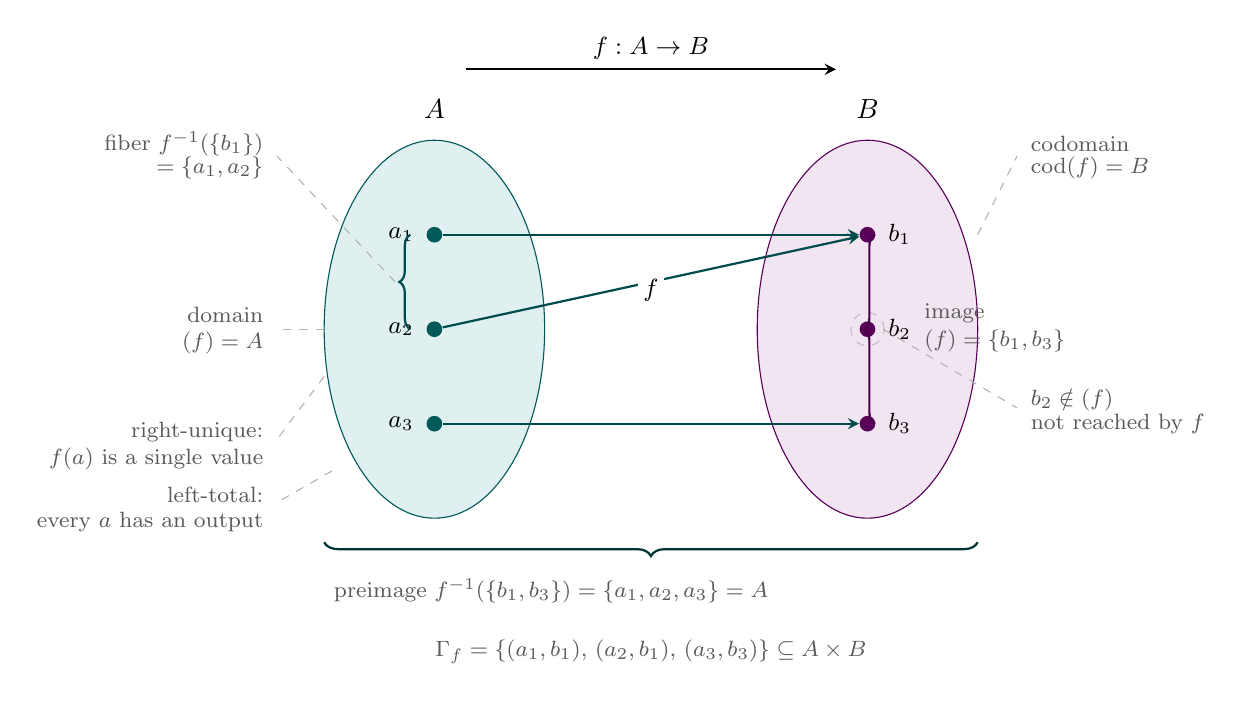
\begin{tikzpicture}[
    >=stealth,
    dot/.style     = {circle, fill, inner sep=2pt},
    teal/.style    = {draw=teal!70!black,  fill=teal!12},
    purple/.style  = {draw=violet!70!black, fill=violet!10},
    lbl/.style     = {font=\small},
    ann/.style     = {font=\footnotesize, text=gray!70!black},
    leader/.style  = {gray!60, dashed, thin},
    arr/.style     = {->, thick, teal!60!black},
    brace/.style   = {decorate,
                      decoration={brace, amplitude=4pt, raise=3pt},
                      thick, violet!60!black}
  ]

  % --- blobs ---
  \draw[teal]   (0,0)   ellipse (1.4cm and 2.4cm);
  \draw[purple] (5.5,0) ellipse (1.4cm and 2.4cm);

  % blob labels
  \node[font=\normalsize\bfseries] at (0,    2.8) {$A$};
  \node[font=\normalsize\bfseries] at (5.5,  2.8) {$B$};

  % --- elements of A ---
  \node[dot, teal!70!black] (a1) at (0,  1.2) {};
  \node[dot, teal!70!black] (a2) at (0,  0)   {};
  \node[dot, teal!70!black] (a3) at (0, -1.2) {};

  \node[lbl, left=4pt] at (a1) {$a_1$};
  \node[lbl, left=4pt] at (a2) {$a_2$};
  \node[lbl, left=4pt] at (a3) {$a_3$};

  % --- elements of B ---
  \node[dot, violet!70!black] (b1) at (5.5,  1.2) {};
  \node[dot, violet!70!black] (b2) at (5.5,  0)   {};
  \node[dot, violet!70!black] (b3) at (5.5, -1.2) {};

  \node[lbl, right=4pt] at (b1) {$b_1$};
  \node[lbl, right=4pt] at (b2) {$b_2$};
  \node[lbl, right=4pt] at (b3) {$b_3$};

  % b2 not in image: dashed ring
  \draw[gray!50, dashed, thin] (b2) circle (6pt);

  % --- arrows ---
  \draw[arr] (a1) -- (b1);
  \draw[arr] (a2) -- (b1);   % two inputs to b1 => not injective
  \draw[arr] (a3) -- (b3);

  % f label on central arrow
  \node[fill=white, inner sep=2pt, font=\small\bfseries] at (2.75, 0.5) {$f$};

  % --- top-level f : A -> B arrow ---
  \draw[->, thick] (0.4, 3.3) -- node[above, font=\small\bfseries] {$f : A \to B$} (5.1, 3.3);

  % ===  LEFT SIDE ANNOTATIONS ===

  % domain
  \draw[leader] (-1.4, 0) -- (-2.0, 0);
  \node[ann, anchor=east] at (-2.05, 0.18) {domain};
  \node[ann, anchor=east] at (-2.05,-0.18) {$\dom(f) = A$};

  % left-total
  \draw[leader] (-1.3,-1.8) -- (-2.0,-2.2);
  \node[ann, anchor=east] at (-2.05,-2.1) {left-total:};
  \node[ann, anchor=east] at (-2.05,-2.45) {every $a$ has an output};

  % right-unique -- left margin, below domain, clear of everything
  \draw[leader] (-1.4, -0.6) -- (-2.0, -1.4);
  \node[ann, anchor=east] at (-2.05,-1.3)  {right-unique:};
  \node[ann, anchor=east] at (-2.05,-1.65) {$f(a)$ is a single value};

  % === RIGHT SIDE ANNOTATIONS ===

  % codomain  -- top right, well clear of image
  \draw[leader] (6.9,  1.2) -- (7.4,  2.2);
  \node[ann, anchor=west] at (7.45, 2.35) {codomain};
  \node[ann, anchor=west] at (7.45, 2.05) {$\mathrm{cod}(f) = B$};

  % image -- mid right, below codomain
  \draw[brace] (5.7, -1.2) -- (5.7,  1.2);
  \node[ann, anchor=west] at (6.1,  0.2) {image};
  \node[ann, anchor=west] at (6.1, -0.15) {$\im(f) = \{b_1, b_3\}$};

  % b2 not in image
  \draw[leader] (5.7, 0) -- (7.4, -1.0);
  \node[ann, anchor=west] at (7.45,-0.9)  {$b_2 \notin \im(f)$};
  \node[ann, anchor=west] at (7.45,-1.2)  {not reached by $f$};

  % fiber of b1: curly brace on LEFT blob, spanning a1 and a2
  \draw[decorate,
        decoration={brace, amplitude=4pt, raise=3pt},
        thick, teal!60!black]
    (-0.2, 0) -- (-0.2, 1.2);
  \draw[leader] (-0.5, 0.6) -- (-2.0, 2.2);
  \node[ann, anchor=east] at (-2.05, 2.35) {fiber $f^{-1}(\{b_1\})$};
  \node[ann, anchor=east] at (-2.05, 2.05) {$= \{a_1, a_2\}$};

  % preimage of T = {b1, b3}  -- bracket under both blobs
  \draw[decorate,
        decoration={brace, amplitude=5pt, raise=3pt, mirror},
        thick, teal!40!black]
    (-1.4,-2.6) -- (6.9,-2.6);
  % label anchored left so it clears the right-unique text
  \node[ann, anchor=north west] at (-1.4,-3.05)
    {preimage $f^{-1}(\{b_1,b_3\}) = \{a_1,a_2,a_3\} = A$};

  % graph label
  \node[ann] at (2.75,-4.1)
    {$\Gamma_f = \{(a_1,b_1),\,(a_2,b_1),\,(a_3,b_3)\} \subseteq A \times B$};

\end{tikzpicture}
\caption{Vocabulary of a function $f : A \to B$.
  Arrows show $f(a_1)=f(a_2)=b_1$ and $f(a_3)=b_3$.
  The element $b_2$ is not in the image; its fiber is empty.
  The fiber over $b_1$ has two elements, showing $f$ is not injective.}
\label{fig:function-vocabulary}
\end{figure}










% ---------------------------------------------------------
% Injective / Surjective / Bijective
% ---------------------------------------------------------


% =========================================================
% Definition — Injective
% =========================================================

\begin{tcolorbox}[title={Definition --- Injective}]
\begin{definition}[Injective]
\label{def:alg-injective}
Let $f : A \to B$. The function $f$ is \textbf{injective} if
\[
\forall a_1, a_2 \in A,\;
\bigl(f(a_1) = f(a_2) \Rightarrow a_1 = a_2\bigr).
\]
\end{definition}
\end{tcolorbox}

\begin{remark*}[Standard quantified statement]
\[
\begin{aligned}
&f \text{ is injective} \\
&\quad\Longleftrightarrow\quad
\forall a_1, a_2 \in A,\;
\bigl(f(a_1) = f(a_2) \Rightarrow a_1 = a_2\bigr).
\end{aligned}
\]
\end{remark*}

\begin{remark*}[Definition predicate reading]
\[
\operatorname{Injective}(f)
\;\colonequiv\;
\forall a_1, a_2 \in A,\;
\bigl(f(a_1) = f(a_2) \Rightarrow a_1 = a_2\bigr).
\]
\end{remark*}

\begin{remark*}[Negated quantified statement]
\[
\begin{aligned}
&f \text{ is not injective} \\
&\quad\Longleftrightarrow\quad
\exists a_1, a_2 \in A,\;
\bigl(a_1 \ne a_2 \;\land\; f(a_1) = f(a_2)\bigr).
\end{aligned}
\]
\end{remark*}

\begin{remark*}[Negation predicate reading]
\[
\neg \operatorname{Injective}(f)
\;\colonequiv\;
\exists a_1 \ne a_2 \text{ in } A
\text{ such that } f(a_1) = f(a_2).
\]
\end{remark*}

\begin{remark*}[Failure modes]
\[
\exists a_1 \ne a_2 \text{ in } A
\text{ such that } f(a_1) = f(a_2).
\]
\end{remark*}

\begin{remark*}[Failure mode decomposition]
\[
\begin{aligned}
\text{Failure 1 (collision): } 
&f(a_1) = f(a_2), \\
\text{Failure 2 (distinct inputs): } 
&a_1 \ne a_2.
\end{aligned}
\]
\end{remark*}

\begin{remark*}[Contrapositive quantified statement]
\[
\begin{aligned}
&f \text{ is injective} \\
&\quad\Longleftrightarrow\quad
\forall a_1, a_2 \in A,\;
\bigl(a_1 \ne a_2 \Rightarrow f(a_1) \ne f(a_2)\bigr).
\end{aligned}
\]
\end{remark*}

\begin{remark*}[Interpretation]
Injectivity means distinct inputs never collide under $f$.
\end{remark*}

% =========================================================
% Definition — Surjective
% =========================================================

\begin{tcolorbox}[title={Definition --- Surjective}]
\begin{definition}[Surjective]
\label{def:alg-surjective}
Let $f : A \to B$. The function $f$ is \textbf{surjective} if
\[
\forall b \in B,\; \exists a \in A,\; f(a) = b.
\]
\end{definition}
\end{tcolorbox}

\begin{remark*}[Standard quantified statement]
\[
\begin{aligned}
&f \text{ is surjective} \\
&\quad\Longleftrightarrow\quad
\forall b \in B,\; \exists a \in A,\; f(a) = b.
\end{aligned}
\]
\end{remark*}

\begin{remark*}[Definition predicate reading]
\[
\operatorname{Surjective}(f)
\;\colonequiv\;
\forall b \in B,\; \exists a \in A,\; f(a) = b.
\]
\end{remark*}

\begin{remark*}[Negated quantified statement]
\[
\begin{aligned}
&f \text{ is not surjective} \\
&\quad\Longleftrightarrow\quad
\exists b \in B \text{ such that }
\forall a \in A,\; f(a) \ne b.
\end{aligned}
\]
\end{remark*}

\begin{remark*}[Negation predicate reading]
\[
\neg \operatorname{Surjective}(f)
\;\colonequiv\;
\exists b \in B \text{ not attained by } f.
\]
\end{remark*}

\begin{remark*}[Failure modes]
\[
\exists b \in B \text{ such that }
\forall a \in A,\; f(a) \ne b.
\]
\end{remark*}

\begin{remark*}[Failure mode decomposition]
\[
\begin{aligned}
\text{Failure (missing output): } 
&b \in B \text{ with no preimage}.
\end{aligned}
\]
\end{remark*}

\begin{remark*}[Interpretation]
Surjectivity means every element of the codomain is achieved as an output.
\end{remark*}

% =========================================================
% Definition — Bijective
% =========================================================

\begin{tcolorbox}[title={Definition --- Bijective}]
\begin{definition}[Bijective]
\label{def:alg-bijective}
Let $f : A \to B$. The function $f$ is \textbf{bijective} if it is both
injective and surjective.
\end{definition}
\end{tcolorbox}

\begin{remark*}[Standard quantified statement]
\[
\begin{aligned}
&f \text{ is bijective} \\
&\quad\Longleftrightarrow\quad
\Bigl[\forall a_1,a_2 \in A,\;
(f(a_1)=f(a_2)\Rightarrow a_1=a_2)\Bigr] \\
&\qquad\qquad\land\;
\Bigl[\forall b \in B,\; \exists a \in A,\; f(a)=b\Bigr].
\end{aligned}
\]
\end{remark*}

\begin{remark*}[Definition predicate reading]
\[
\operatorname{Bijective}(f)
\;\colonequiv\;
\operatorname{Injective}(f)
\;\land\;
\operatorname{Surjective}(f).
\]
\end{remark*}

\begin{remark*}[Negated quantified statement]
\[
\begin{aligned}
&f \text{ is not bijective} \\
&\quad\Longleftrightarrow\quad
(\neg \text{injective}) \;\lor\; (\neg \text{surjective}).
\end{aligned}
\]
\end{remark*}

\begin{remark*}[Negation predicate reading]
\[
\neg \operatorname{Bijective}(f)
\;\colonequiv\;
\neg \operatorname{Injective}(f)
\;\lor\;
\neg \operatorname{Surjective}(f).
\]
\end{remark*}

\begin{remark*}[Failure modes]
\[
\begin{aligned}
&\text{Either collisions occur (not injective)} \\
&\quad\text{or some outputs are missing (not surjective).}
\end{aligned}
\]
\end{remark*}

\begin{remark*}[Failure mode decomposition]
\[
\begin{aligned}
\text{Failure 1: } &\exists a_1 \ne a_2,\; f(a_1)=f(a_2), \\
\text{Failure 2: } &\exists b \in B \text{ with no } a \in A \text{ such that } f(a)=b.
\end{aligned}
\]
\end{remark*}

\begin{remark*}[Interpretation]
A bijection is a perfect pairing between $A$ and $B$: no collisions and no gaps.
\end{remark*}









% ---------------------------------------------------------
% Morphisms
% ---------------------------------------------------------

\subsection{Morphisms}

% ---------------------------------------------------------
% TOOLKIT — Morphisms
% ---------------------------------------------------------

% =========================================================
% Definition — Homomorphism
% =========================================================

\begin{tcolorbox}[title={Definition --- Homomorphism}]
\begin{definition}[Homomorphism]
\label{def:homomorphism}
Let $A$ and $B$ be sets each equipped with algebraic structure.
A function $f : A \to B$ is a \textbf{homomorphism} if it preserves
all operations and relations of the structure.

For a binary operation $\star$:
\[
\forall a_1, a_2 \in A,\;
f(a_1 \star a_2) = f(a_1)\star f(a_2).
\]
\end{definition}
\end{tcolorbox}

\begin{remark*}[Standard quantified statement]
\[
\begin{aligned}
&f \text{ is a homomorphism} \\
&\quad\Longleftrightarrow\quad
\forall a_1,a_2 \in A,\;
f(a_1 \star a_2)=f(a_1)\star f(a_2).
\end{aligned}
\]
\end{remark*}

\begin{remark*}[Definition predicate reading]
\[
\operatorname{Homomorphism}(f)
\;\colonequiv\;
\forall a_1,a_2 \in A,\;
f(a_1 \star a_2)=f(a_1)\star f(a_2).
\]
\end{remark*}

\begin{remark*}[Negated quantified statement]
\[
\exists a_1,a_2 \in A \text{ such that }
f(a_1 \star a_2) \ne f(a_1)\star f(a_2).
\]
\end{remark*}

\begin{remark*}[Negation predicate reading]
\[
\neg \operatorname{Homomorphism}(f)
\;\colonequiv\;
\exists a_1,a_2 \in A \text{ where structure is not preserved}.
\]
\end{remark*}

\begin{remark*}[Failure modes]
\[
f(a_1 \star a_2) \ne f(a_1)\star f(a_2).
\]
\end{remark*}

\begin{remark*}[Failure mode decomposition]
\[
\begin{aligned}
\text{Failure: } 
&f \text{ does not commute with the operation } \star.
\end{aligned}
\]
\end{remark*}

\begin{remark*}[Interpretation]
A homomorphism preserves algebraic structure.
\end{remark*}

% =========================================================
% Definition — Monomorphism
% =========================================================

\begin{tcolorbox}[title={Definition --- Monomorphism}]
\begin{definition}[Monomorphism]
\label{def:monomorphism}
A homomorphism $f : A \to B$ is a \textbf{monomorphism} if it is injective:
\[
\forall a_1,a_2 \in A,\;
(f(a_1)=f(a_2)\Rightarrow a_1=a_2).
\]
\end{definition}
\end{tcolorbox}

\begin{remark*}[Standard quantified statement]
\[
\forall a_1,a_2 \in A,\;
(f(a_1)=f(a_2)\Rightarrow a_1=a_2).
\]
\end{remark*}

\begin{remark*}[Definition predicate reading]
\[
\operatorname{Monomorphism}(f)
\;\colonequiv\;
\operatorname{Homomorphism}(f)
\land
\operatorname{Injective}(f).
\]
\end{remark*}

\begin{remark*}[Negated quantified statement]
\[
\exists a_1 \ne a_2 \text{ such that } f(a_1)=f(a_2).
\]
\end{remark*}

\begin{remark*}[Negation predicate reading]
\[
\neg \operatorname{Monomorphism}(f)
\;\colonequiv\;
\text{collision occurs}.
\]
\end{remark*}

\begin{remark*}[Failure modes]
\[
\exists a_1 \ne a_2 \text{ such that } f(a_1)=f(a_2).
\]
\end{remark*}

\begin{remark*}[Failure mode decomposition]
\[
\begin{aligned}
\text{Failure: } 
&f \text{ identifies distinct elements}.
\end{aligned}
\]
\end{remark*}

\begin{remark*}[Interpretation]
A monomorphism embeds $A$ into $B$ without collapsing elements.
\end{remark*}

% =========================================================
% Definition — Epimorphism
% =========================================================

\begin{tcolorbox}[title={Definition --- Epimorphism}]
\begin{definition}[Epimorphism]
\label{def:epimorphism}
A homomorphism $f : A \to B$ is a \textbf{epimorphism} if it is surjective:
\[
\forall b \in B,\; \exists a \in A,\; f(a)=b.
\]
\end{definition}
\end{tcolorbox}

\begin{remark*}[Standard quantified statement]
\[
\forall b \in B,\; \exists a \in A,\; f(a)=b.
\]
\end{remark*}

\begin{remark*}[Definition predicate reading]
\[
\operatorname{Epimorphism}(f)
\;\colonequiv\;
\operatorname{Homomorphism}(f)
\land
\operatorname{Surjective}(f).
\]
\end{remark*}

\begin{remark*}[Negated quantified statement]
\[
\exists b \in B \text{ such that } \forall a \in A,\; f(a)\ne b.
\]
\end{remark*}

\begin{remark*}[Negation predicate reading]
\[
\neg \operatorname{Epimorphism}(f)
\;\colonequiv\;
\text{missing output}.
\]
\end{remark*}

\begin{remark*}[Failure modes]
\[
\exists b \in B \text{ not attained}.
\]
\end{remark*}

\begin{remark*}[Failure mode decomposition]
\[
\begin{aligned}
\text{Failure: } 
&\text{some } b \in B \text{ has no preimage}.
\end{aligned}
\]
\end{remark*}

\begin{remark*}[Interpretation]
An epimorphism covers the codomain.
\end{remark*}

% =========================================================
% Definition — Isomorphism
% =========================================================

\begin{tcolorbox}[title={Definition --- Isomorphism}]
\begin{definition}[Isomorphism]
\label{def:isomorphism}
A homomorphism $f : A \to B$ is an \textbf{isomorphism} if it is bijective.
\end{definition}
\end{tcolorbox}

\begin{remark*}[Standard quantified statement]
\[
\begin{aligned}
&f \text{ is an isomorphism} \\
&\quad\Longleftrightarrow\quad
(\text{injective}) \land (\text{surjective}).
\end{aligned}
\]
\end{remark*}

\begin{remark*}[Definition predicate reading]
\[
\operatorname{Isomorphism}(f)
\;\colonequiv\;
\operatorname{Bijective}(f)
\land
\operatorname{Homomorphism}(f).
\]
\end{remark*}

\begin{remark*}[Negated quantified statement]
\[
(\neg \text{injective}) \lor (\neg \text{surjective}).
\]
\end{remark*}

\begin{remark*}[Negation predicate reading]
\[
\neg \operatorname{Isomorphism}(f)
\;\colonequiv\;
\text{not bijective}.
\]
\end{remark*}

\begin{remark*}[Failure modes]
\[
\text{collision or missing output}.
\]
\end{remark*}

\begin{remark*}[Failure mode decomposition]
\[
\begin{aligned}
\text{Failure 1: } &\text{not injective} \\
\text{Failure 2: } &\text{not surjective}
\end{aligned}
\]
\end{remark*}

\begin{remark*}[Interpretation]
An isomorphism is a reversible structure-preserving map.
\end{remark*}




% =========================================================
% Definition — Endomorphism
% =========================================================

\begin{tcolorbox}[title={Definition --- Endomorphism}]
\begin{definition}[Endomorphism]
\label{def:endomorphism}
Let $A$ be a set with algebraic structure. An \textbf{endomorphism} of $A$
is a homomorphism from $A$ to itself:
\[
f : A \to A.
\]
\end{definition}
\end{tcolorbox}

\begin{remark*}[Standard quantified statement]
\[
\begin{aligned}
&f \text{ is an endomorphism of } A \\
&\quad\Longleftrightarrow\quad
f : A \to A \text{ and } f \text{ preserves structure}.
\end{aligned}
\]
\end{remark*}

\begin{remark*}[Definition predicate reading]
\[
\operatorname{Endomorphism}(f,A)
\;\colonequiv\;
\operatorname{Homomorphism}(f)
\;\land\;
(f : A \to A).
\]
\end{remark*}

\begin{remark*}[Negated quantified statement]
\[
f \text{ is not an endomorphism}
\;\Longleftrightarrow\;
\text{$f$ is not a homomorphism or } f : A \not\to A.
\]
\end{remark*}

\begin{remark*}[Negation predicate reading]
\[
\neg \operatorname{Endomorphism}(f,A)
\;\colonequiv\;
\neg \operatorname{Homomorphism}(f)
\;\lor\;
f \text{ has wrong domain/codomain}.
\]
\end{remark*}

\begin{remark*}[Failure modes]
\[
\text{Either structure not preserved or wrong codomain.}
\]
\end{remark*}

\begin{remark*}[Failure mode decomposition]
\[
\begin{aligned}
\text{Failure 1: } &\text{not structure-preserving} \\
\text{Failure 2: } &f : A \to B \text{ with } B \ne A
\end{aligned}
\]
\end{remark*}

\begin{remark*}[Interpretation]
An endomorphism is a structure-preserving self-map of $A$.
\end{remark*}

% =========================================================
% Definition — Automorphism
% =========================================================

\begin{tcolorbox}[title={Definition --- Automorphism}]
\begin{definition}[Automorphism]
\label{def:automorphism}
An \textbf{automorphism} of $A$ is a bijective endomorphism:
\[
f : A \to A \quad \text{bijective and structure-preserving}.
\]
\end{definition}
\end{tcolorbox}

\begin{remark*}[Standard quantified statement]
\[
\begin{aligned}
&f \text{ is an automorphism of } A \\
&\quad\Longleftrightarrow\quad
f : A \to A,\;
f \text{ is a homomorphism, injective, and surjective}.
\end{aligned}
\]
\end{remark*}

\begin{remark*}[Definition predicate reading]
\[
\operatorname{Automorphism}(f,A)
\;\colonequiv\;
\operatorname{Endomorphism}(f,A)
\;\land\;
\operatorname{Bijective}(f).
\]
\end{remark*}

\begin{remark*}[Negated quantified statement]
\[
f \text{ is not an automorphism}
\;\Longleftrightarrow\;
\text{not bijective or not structure-preserving}.
\]
\end{remark*}

\begin{remark*}[Negation predicate reading]
\[
\neg \operatorname{Automorphism}(f,A)
\;\colonequiv\;
\neg \operatorname{Bijective}(f)
\;\lor\;
\neg \operatorname{Homomorphism}(f).
\]
\end{remark*}

\begin{remark*}[Failure modes]
\[
\text{collision, missing output, or structure not preserved}.
\]
\end{remark*}

\begin{remark*}[Failure mode decomposition]
\[
\begin{aligned}
\text{Failure 1: } &\text{not injective} \\
\text{Failure 2: } &\text{not surjective} \\
\text{Failure 3: } &\text{not structure-preserving}
\end{aligned}
\]
\end{remark*}

\begin{remark*}[Interpretation]
An automorphism is a symmetry of $A$: a reversible structure-preserving relabeling.
\end{remark*}

% =========================================================
% Definition — Composition
% =========================================================

\begin{tcolorbox}[title={Definition --- Composition}]
\begin{definition}[Composition]
\label{def:alg-composition}
Let $f : A \to B$ and $g : B \to C$. The \textbf{composition}
$g \circ f : A \to C$ is defined by
\[
(g \circ f)(a) := g(f(a)) \quad \text{for all } a \in A.
\]
\end{definition}
\end{tcolorbox}

\begin{remark*}[Standard quantified statement]
\[
\begin{aligned}
&\forall a \in A,\;
(g \circ f)(a) = g(f(a)).
\end{aligned}
\]
\end{remark*}

\begin{remark*}[Definition predicate reading]
\[
\operatorname{Composition}(g,f)(a)
\;\colonequiv\;
g(f(a)).
\]
\end{remark*}

\begin{remark*}[Negated quantified statement]
\[
\exists a \in A \text{ such that }
(g \circ f)(a) \ne g(f(a)).
\]
\end{remark*}

\begin{remark*}[Negation predicate reading]
\[
\neg \operatorname{Composition}(g,f)
\;\colonequiv\;
\text{composition rule fails}.
\]
\end{remark*}

\begin{remark*}[Failure modes]
\[
(g \circ f)(a) \ne g(f(a)).
\]
\end{remark*}

\begin{remark*}[Failure mode decomposition]
\[
\begin{aligned}
\text{Failure: } 
&\text{composition not defined or misapplied}.
\end{aligned}
\]
\end{remark*}

\begin{remark*}[Interpretation]
Composition chains functions: apply $f$ first, then $g$.
\end{remark*}











% ---------------------------------------------------------
% Identity
% ---------------------------------------------------------

% =========================================================
% Definition — Identity Function
% =========================================================

\begin{tcolorbox}[title={Definition --- Identity Function}]
\begin{definition}[Identity Function]
\label{def:alg-identity}
Let $A$ be a set. The \textbf{identity function} on $A$ is the function
$\mathrm{id}_A : A \to A$ defined by
\[
\forall a \in A,\; \mathrm{id}_A(a) = a.
\]
\end{definition}
\end{tcolorbox}

\begin{remark*}[Standard quantified statement]
\[
\forall a \in A,\; \mathrm{id}_A(a) = a.
\]
\end{remark*}

\begin{remark*}[Definition predicate reading]
\[
\operatorname{IdentityFunction}(\mathrm{id}_A,A)
\;\colonequiv\;
\forall a \in A,\; \mathrm{id}_A(a) = a.
\]
\end{remark*}

\begin{remark*}[Negated quantified statement]
\[
\exists a \in A \text{ such that } \mathrm{id}_A(a) \ne a.
\]
\end{remark*}

\begin{remark*}[Negation predicate reading]
\[
\neg \operatorname{IdentityFunction}(\mathrm{id}_A,A)
\;\colonequiv\;
\text{some element is not fixed}.
\]
\end{remark*}

\begin{remark*}[Failure modes]
\[
\exists a \in A \text{ such that } \mathrm{id}_A(a) \ne a.
\]
\end{remark*}

\begin{remark*}[Failure mode decomposition]
\[
\begin{aligned}
\text{Failure: } 
&\text{the map does not return its input}.
\end{aligned}
\]
\end{remark*}

\begin{remark*}[Interpretation]
The identity function leaves every element unchanged and acts as a neutral
element for composition.
\end{remark*}

% =========================================================
% Definition — Inclusion Map
% =========================================================

\begin{tcolorbox}[title={Definition --- Inclusion Map}]
\begin{definition}[Inclusion Map]
\label{def:alg-inclusion}
Let $A \subseteq B$. The \textbf{inclusion map} $\iota : A \to B$ is defined by
\[
\forall a \in A,\; \iota(a) = a.
\]
\end{definition}
\end{tcolorbox}

\begin{remark*}[Standard quantified statement]
\[
\forall a \in A,\; \iota(a) = a.
\]
\end{remark*}

\begin{remark*}[Definition predicate reading]
\[
\operatorname{InclusionMap}(\iota,A,B)
\;\colonequiv\;
(A \subseteq B)
\;\land\;
\forall a \in A,\; \iota(a) = a.
\]
\end{remark*}

\begin{remark*}[Negated quantified statement]
\[
(A \nsubseteq B)
\;\lor\;
\exists a \in A \text{ such that } \iota(a) \ne a.
\]
\end{remark*}

\begin{remark*}[Negation predicate reading]
\[
\neg \operatorname{InclusionMap}(\iota,A,B)
\;\colonequiv\;
\text{not inclusion or not identity-on-domain}.
\]
\end{remark*}

\begin{remark*}[Failure modes]
\[
\begin{aligned}
&A \nsubseteq B
\quad\text{or}\quad
\exists a \in A,\; \iota(a) \ne a.
\end{aligned}
\]
\end{remark*}

\begin{remark*}[Failure mode decomposition]
\[
\begin{aligned}
\text{Failure 1: } &A \text{ not a subset of } B \\
\text{Failure 2: } &\iota \text{ does not act as identity on } A
\end{aligned}
\]
\end{remark*}

\begin{remark*}[Interpretation]
The inclusion map embeds $A$ into $B$ without changing elements.
\end{remark*}

% =========================================================
% Definition — Restriction / Extension
% =========================================================

\begin{tcolorbox}[title={Definition --- Restriction / Extension}]
\begin{definition}[Restriction and Extension]
\label{def:alg-restriction}
Let $f : A \to B$ and $C \subseteq A$.
\begin{enumerate}[label=(\roman*)]
  \item The \textbf{restriction} $f|_C : C \to B$ is defined by
        \[
        \forall c \in C,\; f|_C(c) = f(c).
        \]
  \item A function $g : A' \to B$ is an \textbf{extension} of $f$ if
        $A \subseteq A'$ and
        \[
        \forall a \in A,\; g(a) = f(a).
        \]
\end{enumerate}
\end{definition}
\end{tcolorbox}

\begin{remark*}[Standard quantified statement]
\[
\begin{aligned}
&\forall c \in C,\; f|_C(c) = f(c), \\
&\forall a \in A,\; g(a) = f(a).
\end{aligned}
\]
\end{remark*}

\begin{remark*}[Definition predicate reading]
\[
\begin{aligned}
&\operatorname{Restriction}(f,C)
\;\colonequiv\;
\forall c \in C,\; f|_C(c)=f(c), \\
&\operatorname{Extension}(g,f)
\;\colonequiv\;
(A \subseteq A') \land
\forall a \in A,\; g(a)=f(a).
\end{aligned}
\]
\end{remark*}

\begin{remark*}[Negated quantified statement]
\[
\begin{aligned}
&\exists c \in C \text{ such that } f|_C(c) \ne f(c), \\
&\exists a \in A \text{ such that } g(a) \ne f(a).
\end{aligned}
\]
\end{remark*}

\begin{remark*}[Negation predicate reading]
\[
\neg \operatorname{Restriction}
\;\lor\;
\neg \operatorname{Extension}.
\]
\end{remark*}

\begin{remark*}[Failure modes]
\[
\text{restriction mismatch or extension mismatch}.
\]
\end{remark*}

\begin{remark*}[Failure mode decomposition]
\[
\begin{aligned}
\text{Failure 1: } &f|_C \text{ disagrees with } f \\
\text{Failure 2: } &g \text{ does not extend } f
\end{aligned}
\]
\end{remark*}

\begin{remark*}[Interpretation]
Restriction limits a function to a smaller domain; extension enlarges it
while preserving existing values.
\end{remark*}

% =========================================================
% Definition — Inverses
% =========================================================

\begin{tcolorbox}[title={Definition --- Left/Right Inverse}]
\begin{definition}[Left Inverse, Right Inverse, Inverse]
\label{def:alg-inverse}
Let $f : A \to B$.
\begin{enumerate}[label=(\roman*)]
  \item $g : B \to A$ is a \textbf{left inverse} if
        \[
        \forall a \in A,\; g(f(a)) = a.
        \]
  \item $h : B \to A$ is a \textbf{right inverse} if
        \[
        \forall b \in B,\; f(h(b)) = b.
        \]
  \item $f$ is \textbf{invertible} if there exists $f^{-1}$ satisfying both.
\end{enumerate}
\end{definition}
\end{tcolorbox}

\begin{remark*}[Standard quantified statement]
\[
\begin{aligned}
&\forall a \in A,\; g(f(a))=a, \\
&\forall b \in B,\; f(h(b))=b.
\end{aligned}
\]
\end{remark*}

\begin{remark*}[Definition predicate reading]
\[
\begin{aligned}
&\operatorname{LeftInverse}(g,f)
\;\colonequiv\;
\forall a \in A,\; g(f(a))=a, \\
&\operatorname{RightInverse}(h,f)
\;\colonequiv\;
\forall b \in B,\; f(h(b))=b.
\end{aligned}
\]
\end{remark*}

\begin{remark*}[Negated quantified statement]
\[
\begin{aligned}
&\exists a \in A,\; g(f(a)) \ne a, \\
&\exists b \in B,\; f(h(b)) \ne b.
\end{aligned}
\]
\end{remark*}

\begin{remark*}[Negation predicate reading]
\[
\neg \operatorname{LeftInverse}
\;\lor\;
\neg \operatorname{RightInverse}.
\]
\end{remark*}

\begin{remark*}[Failure modes]
\[
\text{composition fails to return identity}.
\]
\end{remark*}

\begin{remark*}[Failure mode decomposition]
\[
\begin{aligned}
\text{Failure 1: } &g \circ f \ne \mathrm{id}_A \\
\text{Failure 2: } &f \circ h \ne \mathrm{id}_B
\end{aligned}
\]
\end{remark*}

\begin{remark*}[Interpretation]
A left inverse undoes $f$ on inputs; a right inverse undoes $f$ on outputs.
Both together give full reversibility.
\end{remark*}